\section{Fractals}

% FRAME 14
\begin{frame}{Fractals}
	\centering
	\includegraphics[width = 8cm]{Pictures/fractalcover.jpg}
	\end{frame}
	
	% FRAME 15
	\begin{frame}{Motivation}
	\begin{itemize}
		\item Structure of Coastline
		\item Lungs
		
		\centering
		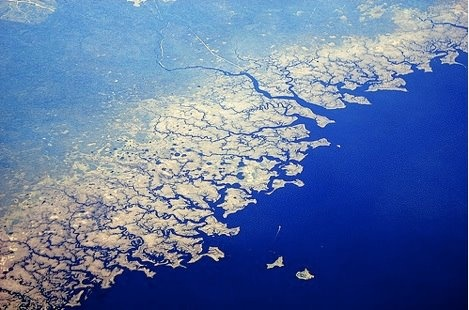
\includegraphics[width = 5cm]{Pictures/coastline.jpg}
		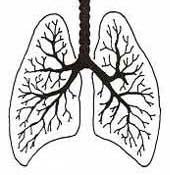
\includegraphics[height = 3.4cm, width  = 4cm]{Pictures/lungs.jpg}
	\end{itemize}
	\end{frame}
	
	% FRAME 16
	\begin{frame}{Some applications}
		\begin{itemize}
			\item Computer simulation: Fractal landscape
			\item Sphere packing: Fractal dimension
	
			\centering
			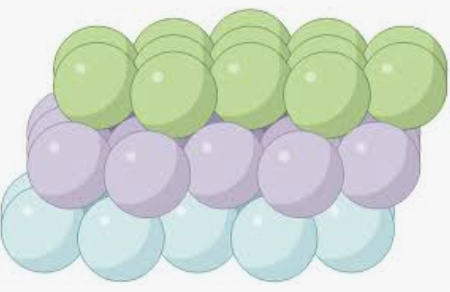
\includegraphics[width=7cm]{Pictures/spherepacking.png}
		\end{itemize}
	\end{frame}


\begin{frame}
	\frametitle{Application}
	\begin{itemize}
		\item Medicine
		\begin{itemize}
			\item Identifying tumors in brain MR images \cite{iftekharuddin2003fractal}
			\item Diabetic retinopathy, etc. : blood vessel's diameter \cite{uahabi2015applications}
		\end{itemize}
		\item Economics
		\begin{itemize}
			\item Market properties, price fluctuation, money flow. \cite{takayasu2009fractals}
		\end{itemize}
		\item Geology and Ecology
		\begin{itemize}
			\item Landscape patterns, vegetation structure, animal habitats. \cite{LOEHLE1996271}
		\end{itemize}
		\item Computer science
		\begin{itemize}
			\item Image encryption. \cite{sangavi2019image}
			\item Computer graphics. \cite{sala2021fractal}
		\end{itemize}
		\item Architecture
		\begin{itemize}
			\item Combining aesthetics and functionality. \cite{lorenz2002fractals}
		\end{itemize}
	\end{itemize}
\end{frame}

\begin{frame}{Fractal Dimension}
	\begin{itemize}
		\item Key Question: How does the object scale?
	\end{itemize}
	\begin{figure}
		\centering
		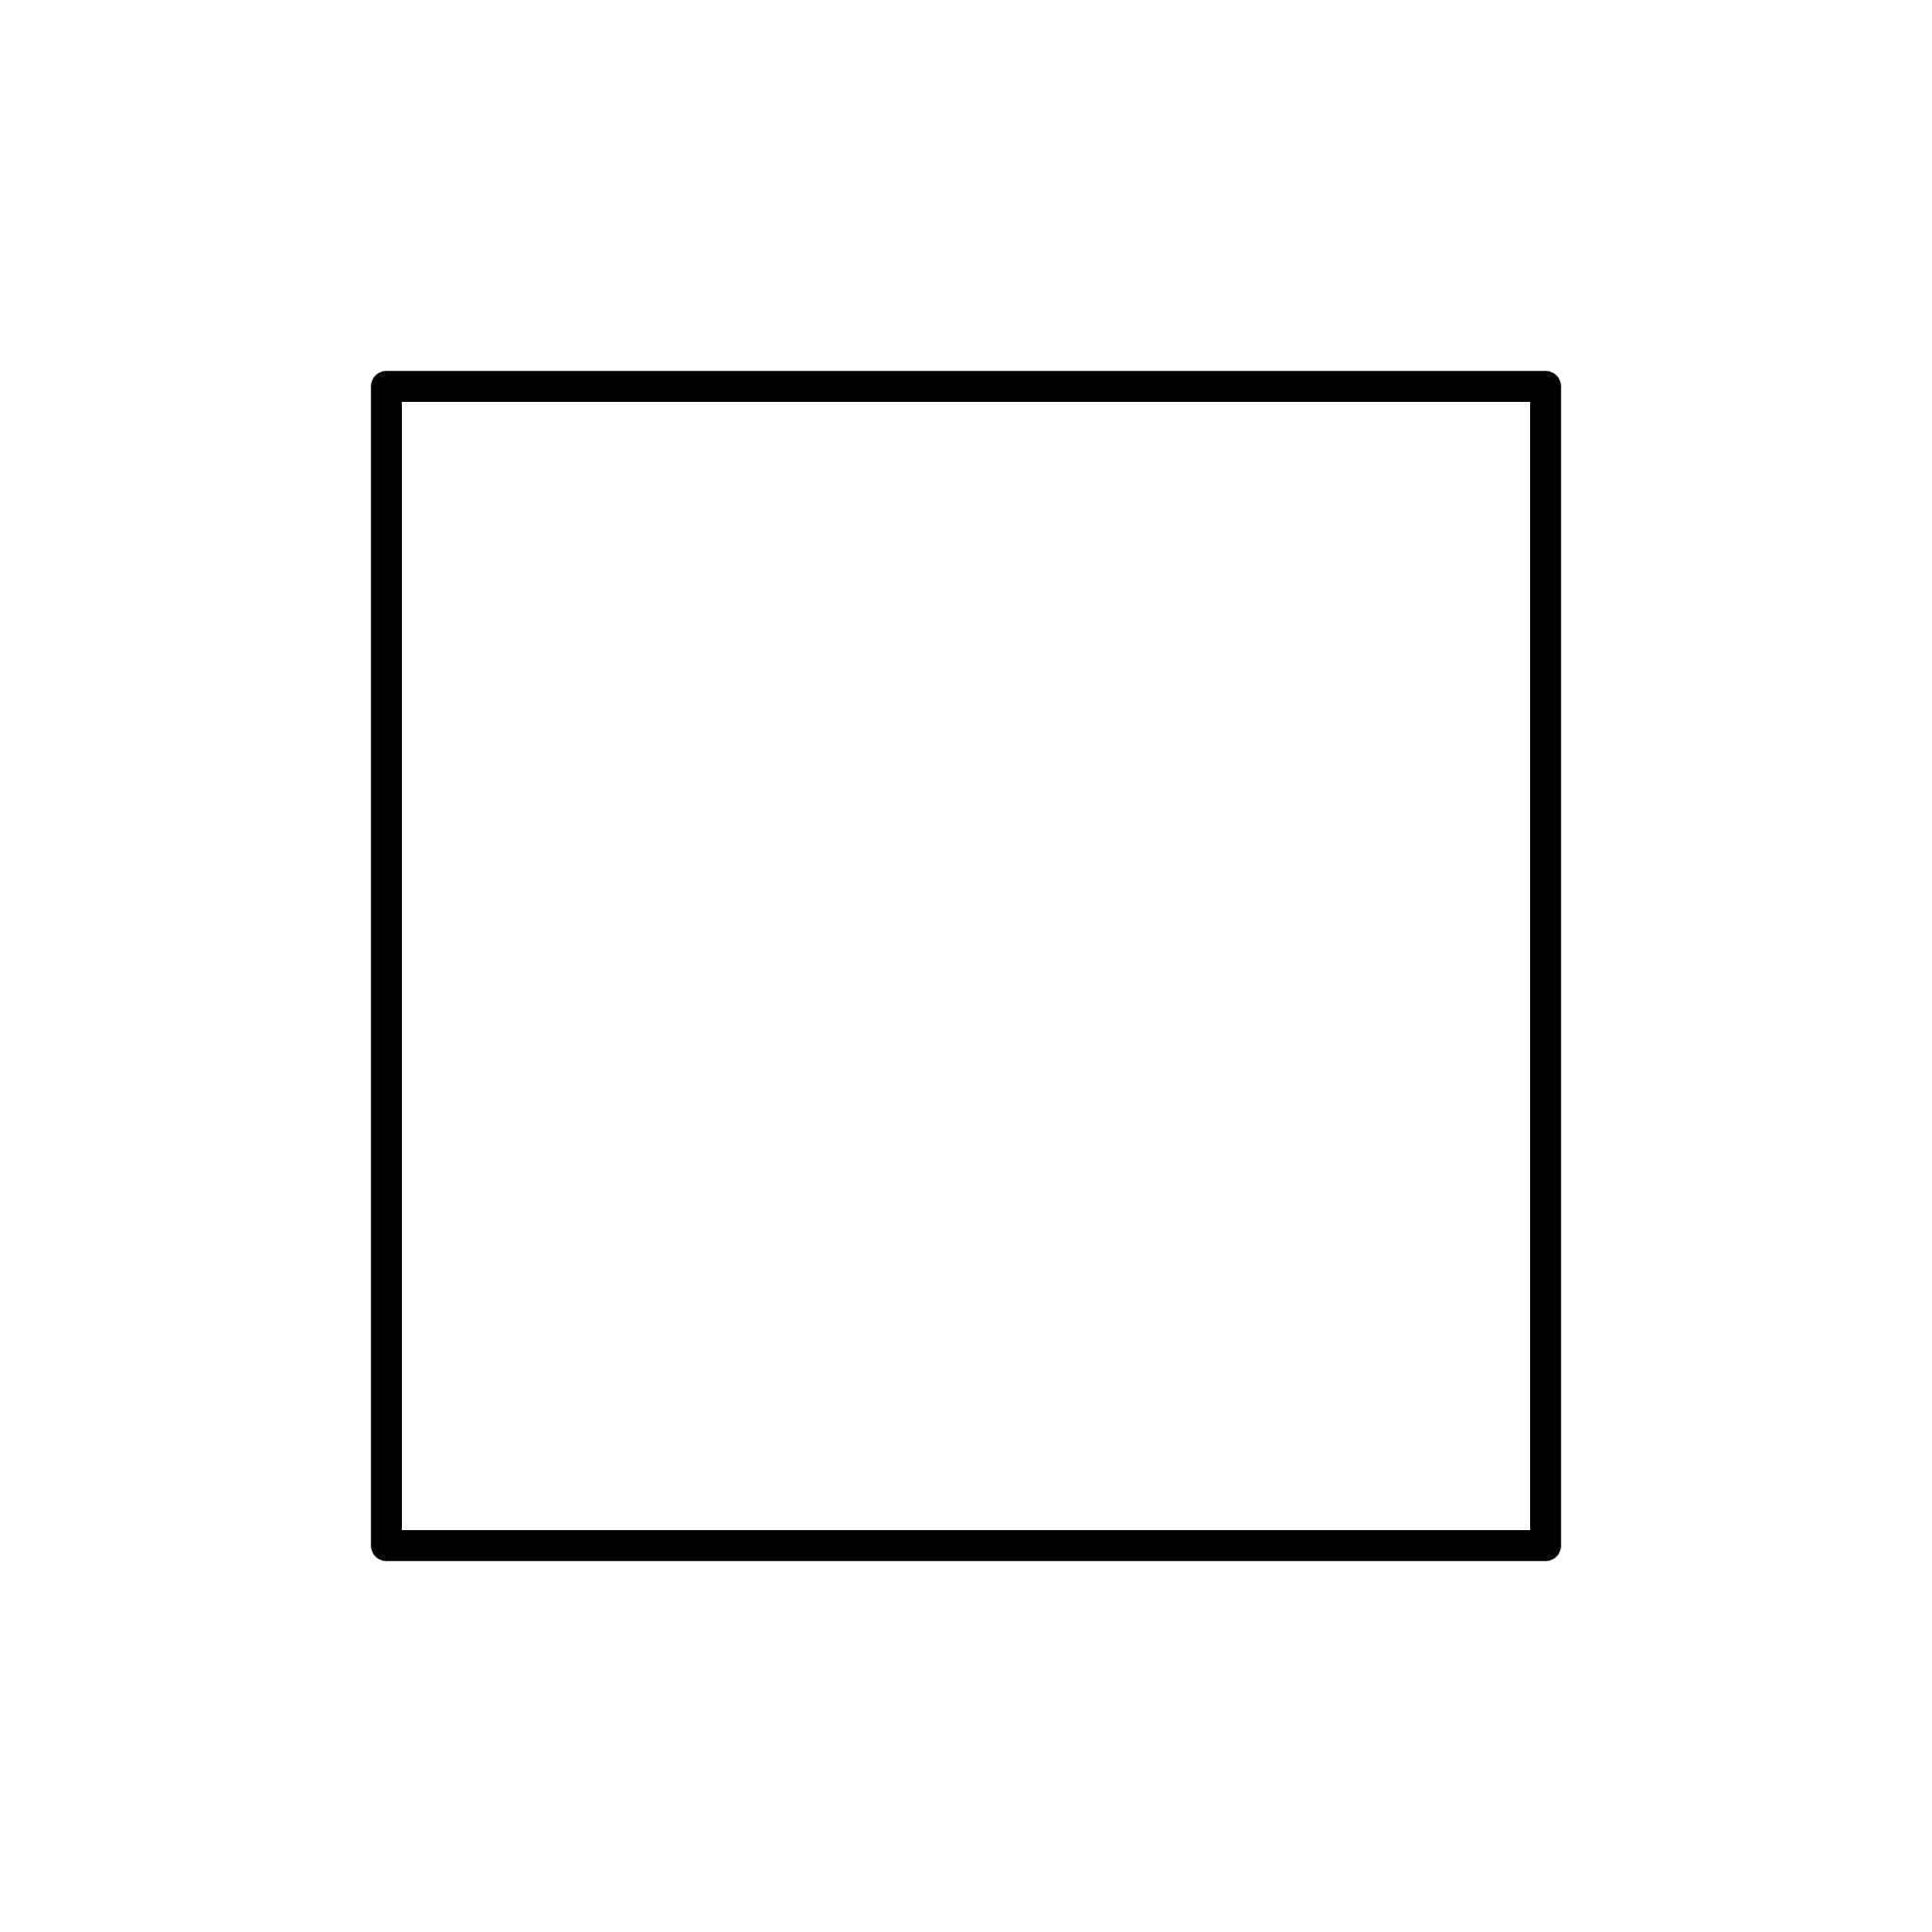
\includegraphics[width=0.25\linewidth]{MichaelImages/Square.png}
		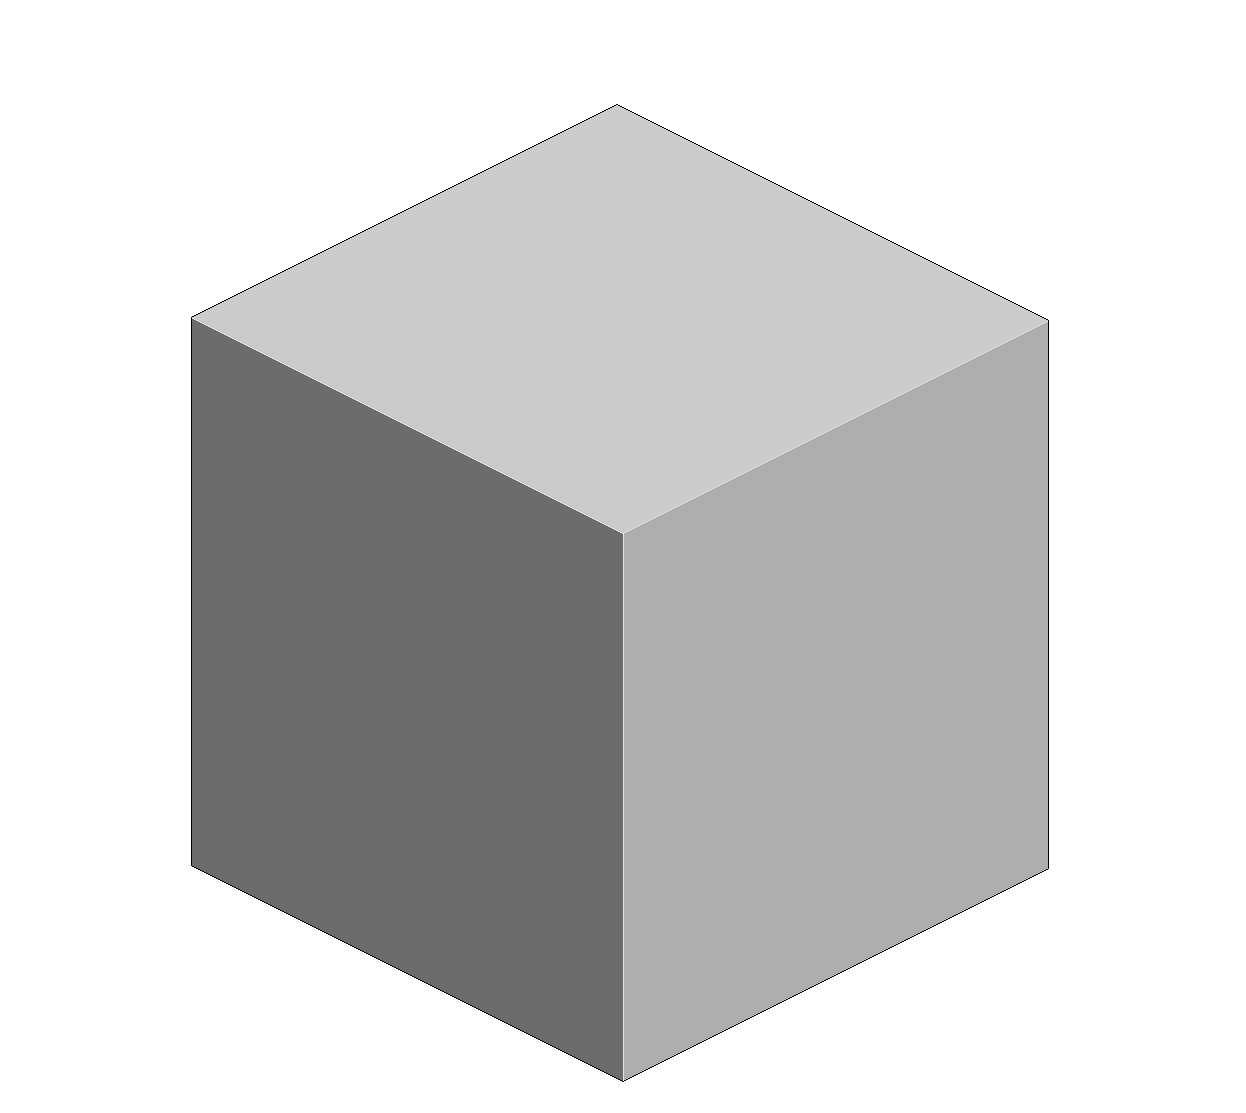
\includegraphics[width=0.25\linewidth]{MichaelImages/3d-cube-transparent-png-4.png}
		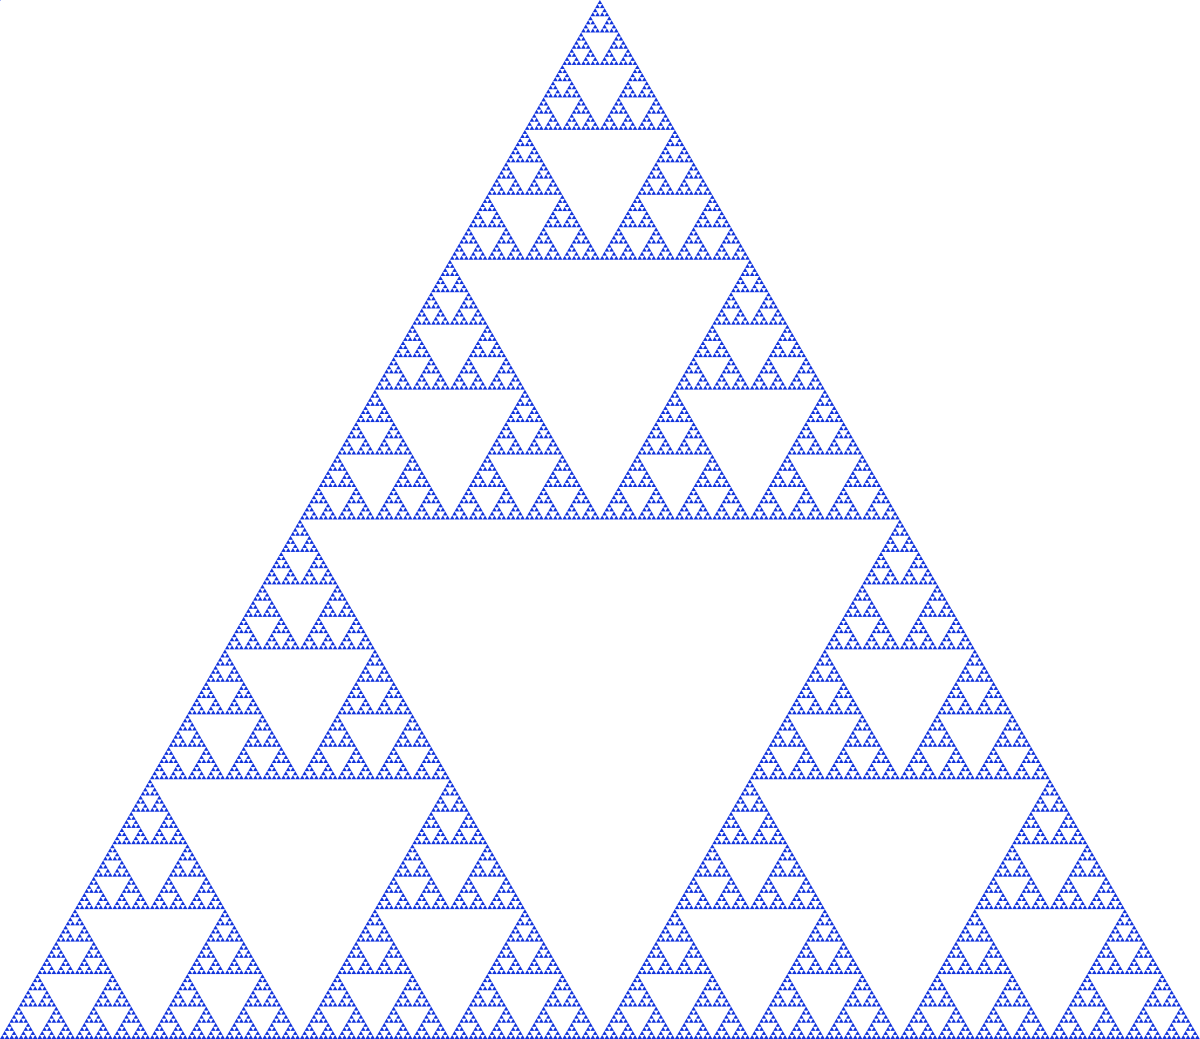
\includegraphics[width=0.25\linewidth]{MichaelImages/Sierpinski_triangle.svg.png}
		\caption{\cite{555w}}
	\end{figure}
	\end{frame}
	
	\begin{frame}{ Minkowski–Bouligand dimension}
	\begin{itemize}
		\item Place our fractal in grid of "boxes"
		\item How does the number of boxes change as they get smaller?
	\end{itemize}
	
	\begin{center}
		\[\dim_{box}(S) = \lim_{\epsilon \to 0}\frac{log (N(\epsilon))}{log(\epsilon^{-1})}\] 
	\end{center}
	\begin{figure}
		\centering
		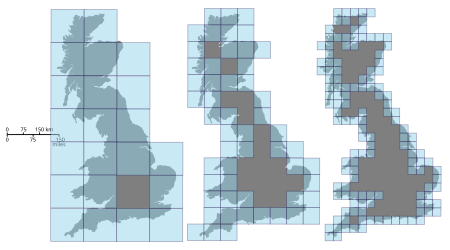
\includegraphics[width=0.25\linewidth]{MichaelImages/Great_Britain_Box.svg.png}
		\caption{\cite{555w}}
		\label{fig:enter-label}
	\end{figure}
	\end{frame}